%!TEX root=./LIVRO.tex
\chapter{Práticas corporais}
\markboth{Módulo 1}{}

\vspace*{-1.5cm}
\enlargethispage{3\baselineskip}

\section*{Habilidades do SAEB}

% \marginnote{Este módulo tem o objetivo de o aluno identificar as principais
% características das práticas corporais reconhecendo as modalidades que
% são definidas como jogos, esportes, lutas, ginásticas e danças.\\

\begin{itemize}
\item
  Identificar elementos constitutivos dos esportes, da ginástica e das
  lutas.
\item
  Identificar a importância do respeito ao oponente e às normas de
  segurança na vivência das práticas corporais (jogos, lutas,
  ginásticas, esportes e dança).
\item
  Analisar os esportes e as lutas nas suas manifestações profissional e
  de lazer.
\item
  Avaliar situações de preconceito no contexto das práticas corporais.
\item
  Avaliar meios para superar situações de preconceito no contexto das
  práticas corporais.
\end{itemize}

\subsection{Habilidades da BNCC}

\begin{itemize}
\item EF35EF03, EF35EF15.
\end{itemize}

%\textless{}Arte: a ideia é fazer um mapa mental com os textos a seguir\textgreater{}

\conteudo{As práticas corporais são todas as ações que fazem com que nosso
corpo se movimente – seja para fazer uma simples tarefa do dia, realizar algum
exercício físico ou praticar alguma modalidade esportiva.

\textbf{Esporte}: atividade voltada para competições que têm regras
fixas e que não podem ser alteradas. Outra característica é que, para os esportes, existem confederações que os
fiscalizam, assim como suas competições.

\textbf{Dança}: atividade em que o praticante usa o corpo para se
expressar por meio de passos, necessariamente com a presença de música.
Também é usada para diversão e socialização, podendo ser realizada
individualmente, em duplas ou em grupos.

\textbf{Luta}: Prática que foi criada para a defesa pessoal e apresenta modalidades com
diferentes golpes (chutes, socos, técnicas de queda etc.). São práticas
que também transmitem, a seus praticantes, ambasamentos filosóficos que, geralmente, pregam justamente a não violência e a convivência pacífica.

\textbf{Ginástica}: prática que tem o objetivo de fortalecer o corpo por
meio de movimentos acrobáticos ou de exercícios físicos, ajudando na saúde
e na qualidade de vida. Pode-se usar algum material (bolas, bastões, halteres,
máquinas etc.) ou apenas o próprio corpo.

\textbf{Jogos e brincadeiras}: atividades que têm semelhanças com alguns
esportes e são voltadas para o lazer e a diversão. Sua principal
característica é que, no jogo, as regras podem ser modificadas. Podem
existir brincadeiras de diferentes culturas, cada uma carregando traços que são transmitidos de pessoaa pessoa dentro de uma comunidade.}

% \coment{É importante que os estudantes saibam
% diferenciar e identificar cada tipo de prática corporal. É possível que
% a turma entenda que tudo está englobado no conceito de “esporte”, mas muitas práticas corporais não
% foram criadas para o aspecto de competição, e sim para diversão ou
% saúde.}

\section*{Atividades}

\num{1} Escreva exemplos de práticas corporais.

\begin{enumerate}
\item
  Esporte: \reduline{futebol, handebol, vôlei.\hfill}
\item
  Lutas: \reduline{judô, karatê, boxe.\hfill}
\item
  Danças: \reduline{samba, tango, valsa, hip-hop.\hfill}
\item
  Ginásticas: \reduline{pilates, yoga, exercícios de musculação.\hfill}
\item
  Jogos e brincadeiras: \reduline{pega-pega, esconde-esconde.\hfill}
\end{enumerate}

% \coment{As respostas são pessoais para cada
% estudante, então podem aparecer outras respostas. Esta atividade tem como
% objetivo analisar o conhecimento prévio deles e identificar se
% sabem diferenciar cada prática corporal.}

\num{2} Qual a principal diferença entre um esporte, como o futebol, e um
  jogo, como a brincadeira do “bobinho”?

\reduline{Os esportes têm regras fixas e são voltados para competições. Já os
jogos (brincadeiras) podem ter suas regras alteradas para promover a
diversão entre os praticantes.\hfill}
\linhas{1}

\num{3} Leia as afirmativas a seguir e marque V para as verdadeiras e F para
  as falsas.

\begin{boxlist}
\boxitem{F} As lutas ajudam as pessoas a brigarem.

\boxitem{V} As danças podem ajudar na socialização, mas também podem ser realizadas individualmente.

\boxitem{F} As ginásticas dificilmente melhoram a qualidade de vida do praticante.

\boxitem{V} As brincadeiras podem ser adaptadas para cada grupo de pessoas.

\boxitem{F} Os esportes têm como função incentivar discussões entre as pessoas.
\end{boxlist}

% \coment{Esta atividade deve ser usada para os
% estudantes identificarem cada atividade em sua prática. Caso seja necessário,
% retome as principais características e os principais exemplos das práticas corporais.}

\num{4} Leia o texto a seguir e complete as lacunas com as palavras que seguem:

\begin{mdframed}[linewidth=2pt,linecolor=salmao,backgroundcolor=salmao!20]
\textbf{Segurança}\hfill
\textbf{Cuidados}\hfill
\textbf{Respeitar}\hfill
\textbf{Regras}\hfill
\textbf{Prática}\hfill
\end{mdframed}

\begin{quote}
Não importa a \preencher{prática} corporal, sempre devemos \preencher{respeitar} as pessoas que
estão participando da atividade, respeitando também as \preencher{regras}. Além
disso, também devemos realizar os devidos \preencher{cuidados} para que a atividade
praticada seja realizada com \preencher{segurança} para ninguém se machucar.
\end{quote}

% \coment{Esta atividade vai ajudar o estudante a
% entender que, em qualquer prática corporal, devem-se seguir as normas, ou
% seja, as regras para promover a segurança e o respeito entre os
% participantes.}


\num{5} Imagine a seguinte situação: um amigo da sua turma começou a praticar
  o hip-hop, mas alguns colegas falam que ele deve parar de dançar. O
  motivo é que falam que as danças só podem ser realizadas pelas
  meninas.

Com base nessa situação, podemos afirmar que existe preconceito?
Justifique sua resposta.

\reduline{Sim, pois o preconceito está no pensamento de achar que
algumas modalidades são exclusivas para meninas ou para meninos.
Esta atividade vai ajudar o estudante a
entender situações preconceituosas que podem surgir nas práticas
corporais.\hfill}

\num{6} Ligue as definições do lazer e da profissão com os exemplos das
  práticas corporais de lutas e de esportes.

\begin{multicols}{2}
Seguir as regras de uma competição

oficial de judô.\medskip

Brincar de esgrima com espadas

de papel.\medskip

Treinar de 6 a 8 horas por dia para

uma partida importante. \medskip

Jogar bola no parque com os amigos.

\columnbreak

Profissão no esporte \bigskip

Lazer no esporte \bigskip

Profissão nas lutas \bigskip

Lazer nas lutas
\end{multicols}

%Como vai aparecer o gabarito desta atividade?

% \coment{Esta atividade vai ajudar o estudante a
% entender que tanto o esporte quanto as lutas podem ser realizados no
% âmbito profissional (realizar várias horas de treino, treinar para uma
% competição e seguir regras etc.) ou para o lazer (diversão com amigos ou
% família, com adaptação de regras e materiais).}

\num{7} Imagine que na sua turma entrou uma colega nova que era de outra escola, mas
  alguns colegas a excluíram durante o recreio e em algumas
  atividades em sala de aula. Sendo assim, escreva uma solução para fazer com
  que, por meio das práticas corporais, essa colega seja incorporada, da forma mais natural possível, à turma.

\reduline{Uma solução é realizar jogos ou brincadeiras com a turma toda
para ajudar na socialização entre os colegas.
Outras respostas podem surgir e devem ser acolhidas.
Esta atividade tem como objetivo o aluno
analisar uma situação preconceituosa (excluir um colega na escola) e
encontrar uma solução para acabar com esse preconceito usando as
práticas corporais.\hfill}

\num{8} Explique como as lutas podem ser compreendidas como riquezas culturais de um povo ou de um grupo.

\reduline{As lutas, ao serem transmitidas, não só representam a transmissão da cultura e da maneira de pensar e agir de um povo como também ajudam na promoção de saberes e de filosofias daquele povo.\hfill}\\
\reduline{O objetivo desta atividade é levar os alunos a refletirem sobre a importância das lutas, com sua enorme variedade, para as culturas daqueles que as praticam.\hfill}
\linhas{1}

\num{9} Por que algumas atividades realizadas na escola, além das aulas de educação física, podem ser consideradas práricas corporais?

\reduline{Atividades do recreio e dos intervalos, como corrida, brincadeiras de roda e pega-pega, por exemplo, trabalham o corpo sem que haja, necessariamente, relação com a aula de Educção Física.\hfill}\\
\reduline{Trata-se de uma boa oportunidade para abrir uma discussão com os alunos sobre como é importante colocar o corpo em movimento, mesmo além das aulas de educação física.\hfill}
\linhas{3}

\num{10} Você pratica regularmente algum esporte, alguma luta, alguma dança ou algum tipo de ginástica? Se sim, conte sobre sua experiência. Se não, cite o que gostaria de praticar.

\reduline{Resposta pessoal. É importante estimular, nas discussões, o hábito de realizar essas atividades, reafirmando sua importância.\hfill}
\linhas{4}


\section*{Treino}

\num{1} Leia o texto a seguir.

\begin{myquote}
{[}\ldots{}{]} Conhecido entre os Xavantes como “tobdaé”, essa é a brincadeira com a
peteca, palavra de origem Tupi que significa “golpear com as mãos”.
Feita com areia, penas, couro ou palha de milho, na brincadeira o
desafio é tocar na peteca sem deixá-la cair no chão. Uma variação dessa brincadeira é tentar acertar a peteca em outro jogador, que deve deixar a
partida se for acertado.{[}\ldots{}{]}

\fonte{Da Redação. Centro de Referências em Educação Integral. 6 brincadeiras indígenas para divertir crianças e aproximar culturas. Disponível em: \emph{https://educacaointegral.org.br/reportagens/6-brincadeiras-indigenas-para-divertir-criancas-e-aproximar-culturas/}.
Acesso em: 13 fev. 2023.}
\end{myquote}

\noindent{}O texto mostra uma atividade para o lazer, pois a prática corporal indígena tem

\begin{escolha}
\item variações de como pode ser realizada.

\item movimentos com golpes de lutas.

\item regras que não podem ser alteradas.

\item materiais oficiais para a prática.
\end{escolha}



\num{2} Leia o texto a seguir, que fala sobre a luta indígena.

\begin{myquote}

{[}\ldots{}{]} Frente a frente, e abaixados para protegerem as pernas, os oponentes
giram em forma circular e se enfrentam primeiro pelo olhar.
Posteriormente, agarram-se para ver quem consegue levantar o adversário
e levá-lo ao chão, encostando as costas no solo {[}\ldots{}{]}

Como não há um juiz, são os próprios atletas que decidem pela vitória,
derrota ou empate: caso em que se soltam um do outro e nenhum dos dois é
derrubado. A vitória é recompensada pelo reconhecimento e respeito das
comunidades indígenas ao vencedor. {[}\ldots{}{]}

\fonte{Brasil. Ministério dos Povos Indígenas. Huka Huka, a luta corporal do Xingu, contribui para manter viva a
cultura indígena no Mato Grosso.
Disponível em: \emph{https://www.gov.br/funai/pt-br/assuntos/noticias/2022-02/huka-huka-a-luta-corporal-do-xingu-contribui-para-manter-viva-a-cultura-indigena-no-mato-grosso}.
Acesso em: 13 fev. 2023.}
\end{myquote}

\pagebreak
\noindent{}Com base no texto, podemos afirmar que a huka-huka é uma luta, pois

\begin{escolha}
\item tem regras que podem ser alteradas durante a prática.

\item prioriza o ganhador da luta com prêmios.

\item incentiva as brigas entres os indígenas.

\item promove o respeito entre os lutadores.
\end{escolha}



\num{3} Leia o texto a seguir.

\begin{myquote}
\textbf{Jogos dos Povos Indígenas}

O critério para a participação desses jogos é a força cultural das
etnias, considerando tradições, como a língua, a dança, os rituais, os
cantos, as pinturas corporais, o artesanato e os esportes tradicionais.
{[}\ldots{}{]}

As lutas corporais são realizadas por homens e mulheres e o esporte está
inserido na cultura tradicional dos povos que o praticam: os povos
indígenas Xinguanos, Bakairis os Huka Hukas e os Xavantes, de Mato
Grosso. {[}\ldots{}{]}

{[}\ldots{}{]} Os lutadores se ajoelham girando em círculo anti-horário
frente ao oponente, até se entreolharem e se agarrarem, tentando
levantar o adversário e derrubá-lo ao chão. Os Karajá do Tocantins já
possuem outro estilo, pois os atletas iniciam a luta em pé, se agarrando
pela cintura, até que um consiga derrubar o outro ao chão. {[}\ldots{}{]}

\fonte{Secretaria da Educação. Jogos dos Povos Indígenas. Disponível em: \emph{http://www.educacaofisica.seed.pr.gov.br/modules/conteudo/conteudo.php?conteudo=218}.
Acesso em: 13 fev. 2023.}
\end{myquote}

\noindent{}Após ler o texto, podemos concluir que as luta indígenas se tornaram um
esporte, pois

\begin{escolha}
\item são realizadas por diferentes etnias indígenas

\item estão presentes em uma competição oficial.

\item apresentam variações para iniciar a luta.

\item têm a presença de pinturas corporais.
\end{escolha}



\chapter{Jogos e brincadeiras}
\markboth{Módulo 2}{}

%\coment{Este módulo tem o objetivo de levar o aluno a reconhecer a importância dos jogos e brincadeiras para o desenvolvimento social e físico da pessoa. Também vai fazer com que ele conheça novas culturas, como a indígena e a africana. O aluno também vai perceber que muitos jogos pré-depsortivos servem como uma iniciação esportiva para alguns esportes.\\

\section*{Habilidades do SAEB}

\begin{itemize}
\item
  Identificar as brincadeiras e os jogos populares como patrimônio
  histórico-cultural.
\item
  Valorizar o patrimônio histórico representado pelas brincadeiras e
  jogos, com ênfase naqueles de origem indígena e africana.
\item
  Analisar o protagonismo do trabalho coletivo na vivência dos jogos
  populares e dos esportes.
\end{itemize}

\subsection{Habilidades da BNCC}

\begin{itemize}
\item EF35EF01, EF35EF06.
\end{itemize}

\conteudo{Os jogos e brincadeiras que realizamos em casa ou na escola trazem
vários benefícios para as pessoas. Tais atividades podem, por exemplo,
ser usadas para promover a participação de todos, ou seja, evitar que
algum colega seja excluído. Outro benefício é ajudar as pessoas a
melhorar suas habilidades motoras, como saltar, correr, rolar, arremessar.
Afinal, trata-se de habilidades essenciais para que as pessoas possam realizar as tarefas do dia a dia.

Além disso, muitas brincadeiras são utilizadas como uma iniciação
esportiva. Um exemplo é a brincadeira de “bobinho” do futebol, uma
atividade em que as pessoas treinam os passes do futebol.

Por fim, muitas brincadeiras são consideradas como um patrimônio
cultural do país. O motivo é que muitas dessas brincadeiras, assim como jogos ou brinquedos,
foram criados na cultura africana ou na cultura indígena, ambas fortemente
presentes no nosso país. Portanto, conhecer uma brincadeira faz com que a
gente conheça um pouco de uma cultura diferente.}

\pagebreak
%https://br.freepik.com/vetores-gratis/criancas-felizes-brincando-de-amarelinha-no-playground\_24558957.htm\#page=2\&query=brincadeira\&position=10\&from\_view=search\&track=sph
\begin{figure}[htpb!]
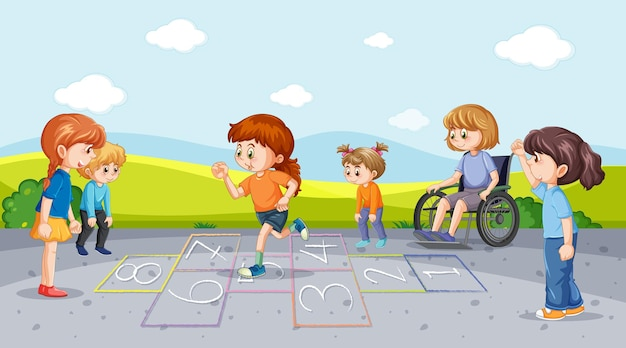
\includegraphics[width=\textwidth]{./imgs/img7.jpg}
\end{figure}

\section*{Atividades}
\enlargethispage{2\baselineskip}

\num{1} A seguir, aparecem algumas brincadeiras populares do Brasil. Escreva a cultura representada por cada brincadeira. Se necessário, peça ajuda ao seu professor.

\begin{enumerate}
\item
  Cabo de guerra: \reduline{Cultura indígena.\hfill}
\item
  Peteca: \reduline{Cultura indígena.\hfill}
\item
  Mancala: \reduline{Cultura africana.\hfill}
\item
  Terra-Mar: \reduline{Cultura africana.\hfill}
\item
  Arco e flecha: \reduline{Cultura indígena.\hfill}
\item
  Jogo da onça: \reduline{Cultura indígena.\hfill}
\item
  Mamba: \reduline{Cultura africana.\hfill}
\end{enumerate}

% \coment{Nesta atividade é muito provável que os alunos precisem de atenção e de direcionamento. Ajude-os, inclusive, propondo, se possível, pesquisa em sala de aula sobre as brincadeiras mencionadas. Caso seja necessário, relembre os estudantes
% de como as brincadeiras apresentadas são realizadas. Esta atividade tem
% como objetivo levar o estudante a identificar a origem de algumas brincadeiras.}

\num{2} Você costuma participar de alguma dessas brincadeiras? Se sim, relate a experiência. Se não, escolha uma que lhe pareça mais divertida e justifique sua escolha.

\reduline{Resposta pessoal\hfill}
\linhas{3}

\num{3} \begingroup
%https://br.freepik.com/vetores-gratis/um-menino-jovem-jogando-voleibol\_5284614.htm\#query=v\%C3\%B4lei\%20kids\&position=10\&from\_view=search\&track=ais
\begin{wrapfigure}{r}{.13\textwidth}
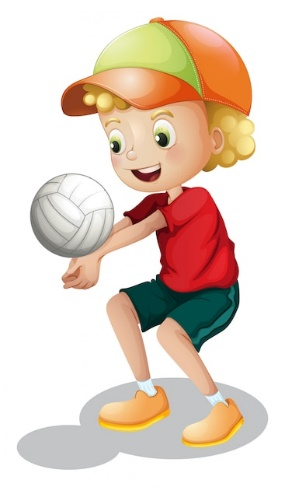
\includegraphics[width=.12\textwidth]{./imgs/img8.jpg}
\end{wrapfigure}

Um jogo popular em algumas escolas é o “3 cortes”. Nesse jogo os
  participantes devem ficar passando a bola entre eles usando as mãos e,
  no terceiro passe (toque), qualquer um pode dar uma cortada para tentar
  acertar alguém.

Depois de ler o texto, reflita: a brincadeira apresenta características de qual
esporte? Justifique sua resposta.

\endgroup\bigskip

\reduline{A brincadeira “3 cortes” é um jogo pré-depsortivo do
voleibol, pelo fato de que, nela, os participantes realizam o
toque e a cortada, dois fundamentos desse esporte.\hfill}\\
\reduline{Os alunos podem escrever outros esportes
que usam a mão para lançar uma bola, como o basquete ou o handebol, mas a
brincadeira apresenta fundamentos do vôlei, que são a cortada e o toque.\hfill}

\num{4} Quais são as brincadeiras mais populares na sua escola?

\reduline{Resposta circunstancial. Ajude os alunos a pensarem em brincadeiras que envolvam mais claramente práticas corporais.\hfill}
\linhas{5}

\pagebreak
\num{5}

\begin{minipage}{.5\textwidth}
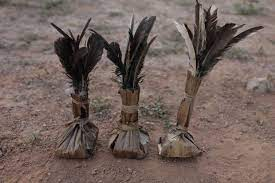
\includegraphics[width=\textwidth]{./imgs/img9.jpg}
\end{minipage}
\hspace{.5cm}
\begin{minipage}{.5\textwidth}
Uma brincadeira comum é a peteca, na qual o objetivo é acetar esse objeto, lançando-o para cima,
  para que não encoste no chão. Existem vários tipos de petecas, mas uma certeza: a de que o objeto foi
  criado pelos povos indígenas. Sendo assim, circule os materiais que
  esses povos podem usar para confeccionar a peteca.
  \end{minipage}\bigskip

\begin{multicols}{2}
\red{Borracha}

\red{Palha}

\red{Folhas}

\blue{Penas de animais}

\blue{Plástico}

\blue{Jornal}
\end{multicols}

%marcar como gabarito para o professor: palha, folhas, penas de animais.

% \coment{Por meio dessa atividade o aluno vai
% entender que muitos objetos usados na atualidade, como a peteca, podem
% ser criados com elementos encontrados na natureza. }

\num{6} Você brinca de peteca? Se sim, usa as mesmas regras mencionadas na atividade anterior? Descreva as regras detalhadamente.

\reduline{Resposta circunstancial.\hfill}
\linhas{4}

\num{7} Leia as afirmativas a seguir e marque V para as verdadeiras e F para
  as falas.

\begin{boxlist}
\boxitem{V} As brincadeiras podem fazer com que as pessoas sejam incluídas.

\boxitem{F} Uma vantagem das brincadeiras é fazer com que as pessoas trabalhem sozinhas.

\boxitem{V} Muitos jogos podem ser usados para aprender um novo esporte.

\boxitem{V} O trabalho em equipe pode ser usado em qualquer brincadeira.

\boxitem{V} O pega-pega é uma brincadeira que ajuda a nossa habilidade motora de correr.
\end{boxlist}

% \coment{Esta atividade tem o objetivo de o aluno
% identificar outras vantagens de praticar uma brincadeira ou jogo
% pré-depsortivo para promover a socialização e o trabalho em equipe.}

\pagebreak
\num{8}

\begin{minipage}{.5\textwidth}
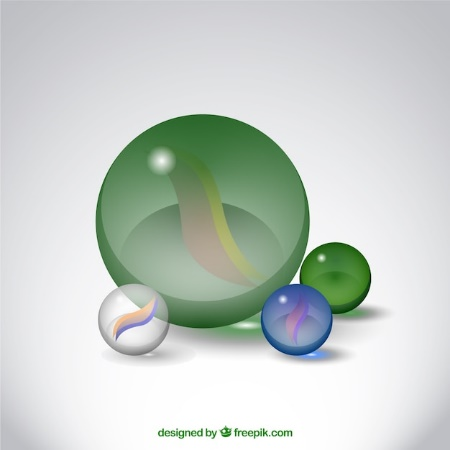
\includegraphics[width=\textwidth]{./imgs/img10.jpg}
%https://br.freepik.com/vetores-gratis/marbles\_797023.htm\#query=marbles\%20ball\&position=2\&from\_view=search\&track=ais
\end{minipage}
\hspace{.5cm}
\begin{minipage}{.5\textwidth}
Ao lado, é apresentada uma ilustração de bolinhas de gude. Trata-se de uma
  brincadeira popular no Brasil, na qual, dependendo da região do país, a
  maneira de brincar pode mudar. Até mesmo o nome da brincadeira pode variar. Por exemplo, no Paraná o brinquedo é chamado de “bola de búrica”, enquanto em Alagoas
  é conhecido como “ximbra”.
\end{minipage}\bigskip

\noindent{}Depois da leitura do texto, punte a afirmação correta sobre a
brincadeira apresentada.

\begin{escolha}
\item
  As características das bolinhas de gude podem variar para cada região
  do país. \rosa{X}
\item
  Somente no Sul do país as bolinhas de gude são conhecidas.
\item
  As regras da brincadeira com bolinha de gude não podem mudar.
\item
  Dependendo do lugar as brincadeiras com bolinhas de gude apenas mudam
  de nome.
\end{escolha}

%\coment{A resposta a ser pintada é a primeira.}

% Por
% meio dessa atividade o aluno vai analisar criticamente que muitas
% brincadeiras podem mudar dependendo da região do país e, por isso, muitas
% atividades são populares no Brasil por serem consideradas um
% patrimônio cultural do país, estando presentes em muitas regiões.}

\num{9} Você acha possível fazer brinquedos com materiais recicláveis? Qual é a importância disso para o meio ambiente?

\reduline{É, sim, possível fazer brinquedos com materiais recicláveis. A importância disso para o meio ambiente é a diminuição de resíduos e a proteção do planeta.\hfill}
\linhas{6}

\pagebreak
\num{10} Faça um desenho que represente a importância dos jogos e das brincadeiras.

\begin{mdframed}[linewidth=2pt,linecolor=salmao]
\coment{Resposta pessoal.}
\vspace{8.5cm}
\end{mdframed}

\section*{Treino}

\num{1} Leia sobre o tag rugby.
\begin{myquote}
  No tag rugby, os jogadores usam um cinto com
  velcro em que está presa uma bandeirola de tecido. Quando essa bandeirinha é retirada
  por um adversário, este é obrigado passar a bola, evitando-se lances violentos.

\fonte{Fonte de pesquisa: Juliana Ribeiro. UmComo. Tag rugby: o que é e regras. Disponível em: \emph{
https://esportes.umcomo.com.br/artigo/tag-rugby-o-que-e-e-regras-30566.html}.
Acesso em: 24 mar. 2023.}
\end{myquote}

\noindent{}Com base no texto, pode-se afirmar que a atividade praticada citada tem o objetivo de

\begin{escolha}
\item desenvolver novos equipamentos esportivos.

\item diminuir brigas e conflitos nos esportes.

\item criar um novo esporte.

\item incentivar a prática de um espore.
\end{escolha}


\pagebreak
\num{2} Leia o texto.

\begin{myquote}
O mancala é um jogo de tabuleiro {[}\ldots{}{]} mais antigo do mundo. É um
recurso lúdico utilizado pela Educação do Acre, em atividade
de contraturno. {[}\ldots{}{]}

O ato de semear, germinação das sementes na terra, desenvolvimento e
colheita são etapas no tabuleiro. Atualmente, é jogado em diversas
partes do mundo e possui mais de 200 variações. “Mancala” significa
mover.

\fonte{Da Redação. Governo do Acre. Mancala: Cultura africana apresentada de forma lúdica.
Disponível em: \emph{
https://agencia.ac.gov.br/mancala-cultura-africana-apresentada-de-forma-ludica/}.
Acesso em: 14 fev. 2023.}
\end{myquote} \enlargethispage{\baselineskip}

\noindent{}Por meio da brincadeira apresentada, podemos

\begin{escolha}
\item adaptar a cultura para a nossa realidade.

\item aprender novas línguas.

\item conhecer tradições de diferentes locais do mundo.

\item estudar uma característica da cultura local.
\end{escolha}



\num{3} Leia um trecho de notícia.

\begin{myquote}
Soltar pipa, jogar bola, pular amarelinha e brincar de pique-esconde
foram algumas das brincadeiras que se tornaram Patrimônio Cultural do
Povo Carioca {[}\ldots{}{]}

{[}\ldots{}{]} o “Poder Executivo, através de seus órgãos competentes, apoiará as iniciativas que visem à valorização e divulgação desta cultura, bem
como oferecerá áreas específicas para que a prática dessas brincadeiras
possa continuar ocorrendo na Cidade” {[}\ldots{}{]}

\fonte{G1. Brincadeiras tradicionais viram Patrimônio Cultural do Povo Carioca;
veja a lista. Disponível em: \emph{
https://g1.globo.com/rj/rio-de-janeiro/noticia/2021/11/05/brincadeiras-tradicionais-viram-patrimonio-cultural-do-povo-carioca-veja-a-lista.ghtml}.
Acesso em: 14 fev. 2023.}
\end{myquote}

\noindent{}Depois da leitura do texto, as brincadeiras citadas se tornaram um
patrimônio para que elas possam

\begin{escolha}
\item ser realizas em alguns lugares do país.

\item ter novas regras e variações.

\item incentivar a venda de materiais para brincar.

\item evitar que as pessoas esqueçam essas atividades.
\end{escolha}




\chapter{Danças indígenas e africanas}
\markboth{Módulo 3}{}

%\coment{Este módulo tem o objetivo de o estudante relembrar as principias características das danças, especialmente as de origens africanas e indígenas, além de identificar os elementos constitutivos da dança (ritmo, espaço, gesto).}

\section*{Habilidades do SAEB}

\begin{itemize}
\item
  Valorizar o patrimônio histórico representado pelas danças populares,
  com ênfase naquelas de matriz indígena e africana.
\item
  Comparar os elementos constitutivos de danças populares do Brasil e do
  mundo com aqueles de danças de matrizes indígena e africana.
\end{itemize}

\subsection{Habilidades da BNCC}

\begin{itemize}
\item EF35EF09, EF35EF10, EF35EF11.
\end{itemize}

\conteudo{As danças são práticas corporais que utilizam os movimentos do corpo para
as pessoas se expressarem e se comunicarem. Mesmo existindo diferentes tipos de
dança, todas elas têm três elementos comuns, que são:

\begin{itemize}
\item
  Ritmo: são as batidas fortes da música para que o dançarino possa
  realizar os movimentos de maneira coordenada e harmoniosa.
\item
  Espaço: é o trajeto que o corpo realiza ao dançar, dando a
  liberdade de a pessoa se movimentar para onde ela quiser. É próprio para
  cada um.
\item
  Gesto: são os passos de dança, que podem conter saltos, giros,
  movimentos acrobáticos. Os gestos podem ser padronizados, criados pelo
  próprio dançarino, e podem ser realizados em grupos ou
  individualmente.
\end{itemize}

É comum as pessoas conhecerem danças de outros lugares, como o tango, a
valsa etc., mas no Brasil existem muitas danças que surgiram aqui mesmo,
como o samba, o forró, entre outras. Uma curiosidade é que, no país,
existem muitas danças de origem africana e indígena.

Também devemos saber que as danças trazem vários benefícios, como cuidar
da saúde e interagir com outras pessoas.}

%https://br.freepik.com/vetores-gratis/pacote-de-silhuetas-de-danca-de-silhuetas-de-dancarinas_23885929.htm\#query=dan\%C3\%A7a\&position=1\&from_view=search\&track=sph
\begin{figure}[htpb!]
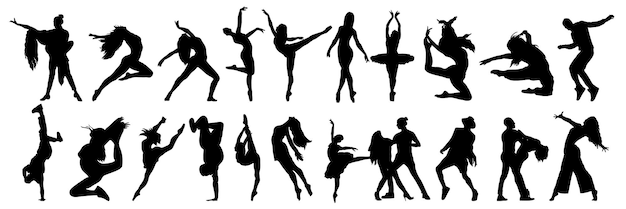
\includegraphics[width=\textwidth]{./imgs/img11.png}
\end{figure}

\section*{Atividades}

\num{1} Relacione as danças da primeira coluna com suas respectivas culturas de
  origem, que estão na segunda coluna.

\begin{multicols}{2}
(\rosa{2}) Toré

(\rosa{2}) Kuarup

(\rosa{1}) Samba

(\rosa{1}) Cateretê

(\rosa{2}) Maracatu

(\rosa{1}) Maculelê

\columnbreak

(1) Cultura africana\medskip

(2) Cultura indígena
\end{multicols}

% \coment{Esta atividade tem a finalidade de levar o aluno a
% identificar e relembrar as danças que são das matrizes indígena ou
% africana.}

\num{2} Você tem conhecimentos de alguma das danças mencionadas na atividade anterior? Se sim, como é sua relação com essa dança? Se não, qual delas gostaria de conhecer melhor?

\reduline{Resposta pessoal.\hfill}
\linhas{3}

\num{3} Na sua escola as pessoas costumam dançar na hora do intervalo ou em festas específicas? Relate esse costume.

\reduline{Resposta pessoal.\hfill}
\linhas{3}

\num{4} Complete o texto a seguir com as palavras que estão faltando.

\begin{quote}
Não importa o tipo de dança, se é indígena, europeia ou africana, todas
elas têm algumas semelhanças!
Sabe aquelas batidas fortes que escutamos em uma música? Isso é o \preencher{ritmo}.
Ele é algo muito importante para que o dançarino consiga realizar o \preencher{gesto} de
uma determinada dança. Por fim, o praticante também deve prestar atenção ao
\preencher{espaço} para que ele possa se movimentar na melhor maneira possível.
\end{quote}

% \coment{A atividade serve como uma fixação para que
% o estudante consiga identificar e diferenciar os três elementos
% constitutivos da dança.}

\num{5} Você já foi a um musical? Nesse tipo de espetáculo, acontecem encenações, como em um teatro, juntamente com canto e dança. Imagine um cenário para um espetáculo musical com alguma das danças mencionadas anteriormente. Desenhe um cenário que combine com esse espetáculo e, em seguida, explique a associação entre o tema proposto e seu desenho.

\begin{mdframed}[linewidth=2pt,linecolor=salmao]
\coment{A associação deve ser coerente, mas não se deve exigir muito conhecimento dos alunos em relação à dança escolhida.}
\vspace{11cm}
\end{mdframed}\pagebreak

\num{6} Observe a imagem e assinale V para as afirmativas verdadeiras e F para as falsas.

\begin{figure}[htpb!]
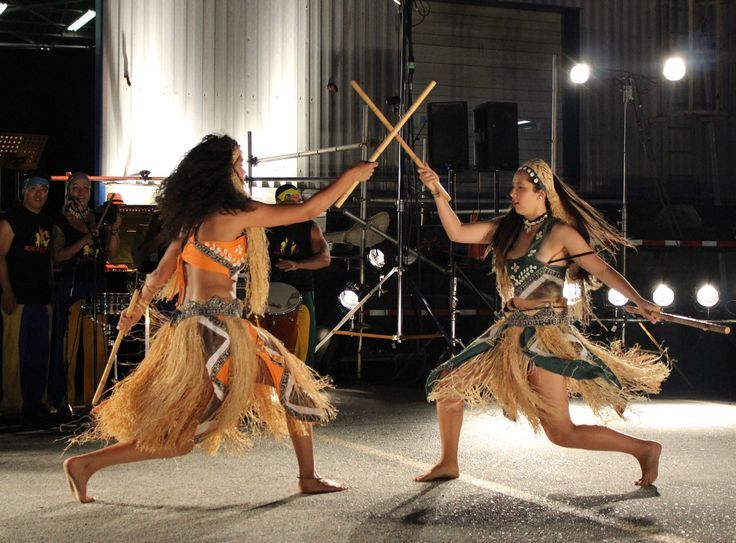
\includegraphics[width=\textwidth]{./imgs/img12.jpg}
\end{figure}

\begin{boxlist}
\boxitem{V} A ilustração mostra o maculelê.

\boxitem{F} As pessoas da imagem estão realizando uma luta.

\boxitem{V} Uma característica é o uso de bastões de madeira.

\boxitem{F} A prática corporal apresentada é de origem indígena.
\end{boxlist}

% \coment{Essa atividade vai ajudar o estudante a
% reconhecer as principais características de uma dança de origem
% africana.}

%https://br.freepik.com/vetores-gratis/plano-de-fundo-do-carnaval-brasileiro\_3872754.htm\#query=samba\&position=8\&from\_view=search\&track=sph

\num{7}

\begin{minipage}{.3\textwidth}

\includegraphics[width=\textwidth]{./imgs/img13.jpg}
\end{minipage}
\hspace{.5cm}
\begin{minipage}{.7\textwidth}
Sabe qual é a dança mais popular no Brasil? Se pensou no samba, você
  acertou! É reconhecida internacionalmente como uma dança
  afro-brasileira e está presente em algumas festas populares no país.
  Além disso, as pessoas se organizam em um grande círculo para dançar e
  tocar alguns instrumentos musicais, como o cavaquinho e o pandeiro.
\end{minipage}\bigskip

\noindent{}Com base no texto, responda às questões a seguir.


\begin{escolha}
\item Por que o samba é conhecido como dança afro-brasileira?\\
\reduline{O samba foi criado pelos negros escravizados que chegaram ao Brasil e
que tinha, desde sempre, influências da cultura brasileira.\hfill}

\item Em qual festa o samba é realizado de forma mais frequente?\\
\reduline{No carnaval.\hfill}

\item Qual o nome da dança de samba em que as pessoas formam um círculo?\\
\reduline{Samba de roda ou roda de samba.\hfill}
\end{escolha}

% \coment{Por meio desta atividade é possível o
% estudante perceber como o samba está presente na cultura brasileira e
% relembrar algumas características dessa dança.}

\num{8} Por que uma dança é considerada uma prática corporal?

\reduline{Uma dança é considerada uma prática corporal poque, para que ela seja praticada, trabalha-se com o corpo.\hfill}
\linhas{3}

\num{9} Use o espaço a seguir para representar uma dança indígena ou uma dança
  africana por meio de uma colagem. Procure representar como são realizados
  os passos de dança, as vestimentas usadas e escreva o nome da dança
  que foi representada.

\begin{mdframed}[linewidth=2pt,linecolor=salmao]
\coment{As representações elaborados pelos alunos vão
ajudá-los a fixar algumas características da dança escolhida, bem como refletirem sobre sua origem.}
\vspace{5cm}
\end{mdframed}

\num{10} Você acha que danças de tradição africana devem ser praticadas apenas por descendentes de pessoas de países africanos? Por quê?

\reduline{Todas as respostas devem ser acolhidas, mas é importante mostrar aos alunos que, quanto mais pessoas praticarem uma dança, melhor para a divulgação dessa cultura e dessa dança.\hfill}
\linhas{3}

\section*{Treino}

\num{1} Leia o texto.
\begin{myquote}
  {[}\ldots{}{]} A dança do \emph{toré} apresenta variações de ritmos e toadas
  dependendo de cada povo. O \emph{maracá} – chocalho indígena feito de
  uma cabaça seca, sem miolo, na qual se colocam pedras ou sementes –
  marca o tom das pisadas e os índios dançam, em geral, ao ar livre e em
  círculos. O ritual do \emph{toré} é considerado o símbolo maior de
  resistência e união entre os índios
  do Nordeste brasileiro. {[}\ldots{}{]}

\fonte{Lúcia Gaspar. Fundação Joaquim Nabuco. Danças indígenas do Brasil. Disponível em: \emph{
http://basilio.fundaj.gov.br/pesquisaescolar/index.php?option=com\_content\&view=article\&id=839:dancas-indigenas-do-brasil\&catid=39:letra-d}.
Acesso em: 14 fev. 2023.}
\end{myquote}

\noindent{}Assim como qualquer dança, a prática corporal indígena citada pode ser assim classificada por

\begin{escolha}
\item variar para cada povo indígena que existe no Brasil.

\item ter instrumentos musicais para ditar o ritmo da dança.

\item ser realizada em locais abertos.

\item promover a interação entres os indígenas.
\end{escolha}


\num{2} Leia com atenção infomações sobre o jongo.

\begin{myquote}
Considerado, desde 2005, patrimônio cultural do Brasil pelo Iphan, o
  jongo conta agora com um centro cultural de 2 mil metros quadrados aos
  pés do Morro da Serrinha, em Madureira, zona norte do Rio. {[}\ldots{}{]}

O jongo chegou ao Brasil com os escravizados africanos de origem bantu,
vindos do Congo e de Angola, permanecendo presente entre aqueles que
trabalhavam nas lavouras de café e cana-de-açúcar no vale do Rio
Paraíba, entre São Paulo e Minas Gerais. Os proprietários das fazendas
permitiam que seus escravos dançassem jongo nos dias dos santos {[}\ldots{}{]}

\fonte{Larissa Altoé. MultiRio. Jongo, expressão da cultura afro-brasileira. Disponível em: \emph{
https://shorturl.at/wFGPS}.
Acesso em: 14 fev. 2023.}
\end{myquote}

\noindent{}Com base no texto, a dança apresentada é de origem africana, pois ela

\begin{escolha}
\item foi criada pelos negros escravizados.

\item surgiu no Sudeste do Brasil.

\item era praticada pelos fazendeiros de café.

\item estava relacionada com eventos religiosos.
\end{escolha}


\num{3} Leia sobre o samba de roda.
\begin{myquote}
O Samba de Roda no Recôncavo Baiano foi reconhecido como Patrimônio Cutural Imaterial da Humanidade.

Essa prática, hoje em dia, envolve e reúne tradições que se transmitem de geração a geração, desde os africanos escravizados até os dias de hoje. Algumas das tradiçõs envolvidas nesse samba de roda são: culto aos orixás e caboclos, jogo da capoeira e “comida de azeite”.

O que também surpreende nesse samba é como ele, vindo da África, se mesclou com a cultura trazida pelos portugueses (como o uso da viola e do pandeiro), além, claro, do uso da língua portuguesa com toda a sua potência.


\fonte{Brasil. Ministério da cultura. Samba de Roda do Recôncavo Baiano completa 18 anos como Patrimônio Cultural do Brasil. Disponível em: \emph{
https://shorturl.at/tvxA3}. Acesso em: 25 mar. 2023.}
\end{myquote}

\noindent{}Depois da leitura do texto, é possível entender que a pessoa que pratica o samba vai

\begin{escolha}
\item realizar uma luta africana.

\item reconhecer costumes alimentares de origem europeia.

\item entender como uma atividade se torna um patrimônio.

\item conhecer diferentes culturais por meio da dança.
\end{escolha}

